\chapter{Forward Model}
\label{ch:formodel}
In this chapter we present the forward model to which we apply all our methodology on. We follow the MIPAS handbook \cite{mipas2000handbook} and simulate data according to a cloud-free atmosphere in local thermodynamic equilibrium and assume a measurement instrument with infinite spectral resolution and no pointing errors.
\begin{figure}[ht!]
	\centering
	\input{LIMB.pdf_tex}
	\caption[Schematic of measurement and analysis geometry.]{Schematic of measurement and analysis geometry, not to scale.
		The stationary satellite, at a constant height $h_\text{sat}$ above Earth, takes $m = 41$ measurements along its line-of-sight defining by the line $\Gamma_j$.
		Each measurement has a limb height $\ell_j$, $j=1,2,\dots,m$ defined as the closest distance of $\Gamma_j$ to the Earth surface.
		Between $h_{L,0} = 7$km and $h_{L,n} = 83.3$km, the stratosphere is discretised into $n =44$ layers as illustrated by the solid green lines.}
	\label{fig:LIMB}
\end{figure}


A satellite at a constant height $h_{\text{sat}}$ points through the atmosphere (limb-sounding) and measures thermal radiation of gas molecules along its line of sight, see  Figure~\ref{fig:LIMB}.
One measurement of the thermal radiation if we target one specific molecule, in our case ozone denoted by the ozone volume mixing ratio $x(r)$ at distance $r$ from the satellite, of at the wave number $\nu$ is given by the path integral
\begin{align}
	\label{eq:RTE} 
	y_j =   \int_{\Gamma_j}  B(\nu,T) k(\nu, T)   \frac{p(T)}{k_{\text{B}} T(r)}  x(r)  \tau(r) \text{d}r + \eta_j \, \\
	\tau(r) = \exp{ \Bigl\{ - \int^{r}_{r_\text{obs}}  k(\nu, T)   \frac{p(T)}{k_B T(r^{\prime})}  x(r^{\prime}) \text{d}r^{\prime} \Bigr\} } \, ,\label{eq:absRTE} 
\end{align}
which is the radiative transfer equation (RTE)~\cite{mipas2000handbook} where we define a tangent height $h_{\ell_j}$ and a pointing direction is $\Gamma_j$ for each $j=1,2,\ldots,m$ measurement of the data vector $\bm{y} \in \mathbb{R}^m$ including some noise $\eta_j$.
Within the atmosphere the number density $p(T) / (k_{\text{B}} T(r))$ of molecules is dependent on the pressure $p(T)$, the temperature $T(r)$, and the Boltzmann constant $k_{\text{B}}$.
The factor $\tau(r)\leq 1$ accounts for re-absorption of the radiation along the line-of-sight, which makes the RTE non linear.
The absorption constant
\begin{align}
	k(\nu, T) = L(\nu, T_{\text{ref}}) \frac{Q(T_{\text{ref}})}{Q(T)} \frac{ \exp{\{ - c_2 E^{\prime \prime} / T\}} }{\exp{\{ - c_2 E^{\prime \prime} / T_{\text{ref}} \}}} \frac{ 1- \exp{\{ - c_2 \nu  / T \}} }{1 - \exp{\{ - c_2 \nu / T_{\text{ref}} \}}}
\end{align}
is depend on the line intensity $L(\nu, T_{\text{ref}})$ at reference temperature $T_{\text{ref}} =296K $, the lower-state energy of the transition $ E^{\prime \prime} $, the second radiation constant $c2=1.4387769\text{cmK}$ all provided by the HITRAN database \cite{gordon2022hitran2020}.
The total internal partition function for the lower-state energy is
\begin{align}
	Q(T )= g^{\prime \prime} \exp{\{ - \frac{ c_2 E^{\prime \prime} }{T}\}} \, ,
\end{align}
with the statistical weight $ g^{\prime \prime}$ (also called the degeneracy factor) accounting for the molecules non-rotational and rotational energy states, see \cite{vsimevckova2006einstein}.
Under the assumption of local thermodynamic equilibrium (LTE) the black body radiation act as a source function
\begin{align}
	B(\nu,T)   = \frac{2 h c^2 \nu^3}{\exp{\{\frac{hc\nu}{k_B T}\}}-1}\, ,
\end{align}
with Planck's constant $h$ and velocity of light $c$ \cite{}.
For fundamentals on the Radiative transfer equation we recommend \cite[Chapter 1]{rybicki2000rte}.

To enable matrix-vector multiplication, we discretise the atmosphere in $n$ layers, where the $i^\text{th}$ layer is defined by two spheres of radii $h_{L,i-1} < h_{L,i}$, for $i = 1, \dots, n$, with $h_{L,0}$ and $h_{L,n} $.
Then we can discretise the ozone, pressure and temperature profiles as a function of height, where in between the heights $h_{L,i-1}$ and $h_{L,i}$, each of the ozone concentration $x_{i}$, the pressure $p_{i}$, the temperature $T_{i}$, as well as the thermal radiation is assumed to be constant.
Above $h_{L, n}$ and below $h_{L,0} $, the ozone concentration is set to zero, so no signal can be obtained.
Depending on the parameter of interest, which is either the ozone volume mixing ratio $\bm{x} =\{x_1,x_2,\ldots,x_n\} \in \mathbb{R}^{n}$ or the fraction of pressure and temperature $\bm{p/T}= \{p_1/T_1,p_2/T_2,\ldots,p_n/T_n\} \in \mathbb{R}^{n} $
we rewrite the integral in Eq.~\eqref{eq:RTE} for one noise free measurement using the trapezoidal rule as a vector-vector multiplication $\bm{A_{j}}(\bm{x},  \bm{p},\bm{T}) \, \bm{x} $ or $\bm{A_{j}}(\bm{x},  \bm{p},\bm{T}) \, \bm{p}/ \bm{T} $, where the non-linear absorption $\tau(r)$ is included in $\bm{A_{j}}(\bm{x},  \bm{p},\bm{T}) \in \mathbb{R}^{n}$ which is the $j$-th row of the matrix $\bm{A}(\bm{x},  \bm{p},\bm{T})$.
Then given a noise vector $\bm{\eta} \in \mathbb{R}^{m}$ the data vector
\begin{align}
	\bm{y} = \bm{A}_{NL} \, \bm{x} + \bm{\eta}= \bm{A}_{NL} \,
	\frac{ \bm{p}}{\bm{T}} + \bm{\eta} \, 
\end{align}
is based on a matrix-vector multiplication, where we define $\bm{A}(\bm{x},  \bm{p},\bm{T}) \equiv \bm{A}_{NL} \in \mathbb{R}^{m \times n}$ for simplicity so that $\bm{A}_{NL}\bm{x}$ or $\bm{A}_{NL}\bm{p}/\bm{T}$ implies the construction of $\bm{A}_{NL}$.
If we neglect the absorption, e.g. set $\tau = 1$ in Eq.~\eqref{eq:absRTE}, this problem becomes a linear problem with the forward model given by $\bm{A}_{L}\bm{x}$ or $\bm{A}_{L}\bm{p}/\bm{T}$. 
Further, we classify the inverse problem as weakly non-linear, see e.g. Fig. \ref{fig:MapAsses}, as neglecting the absorption changes the measurement only slightly.

\section{Singular value decompostion of linear forward model matrix}
\begin{figure}[ht!]
	\centering
	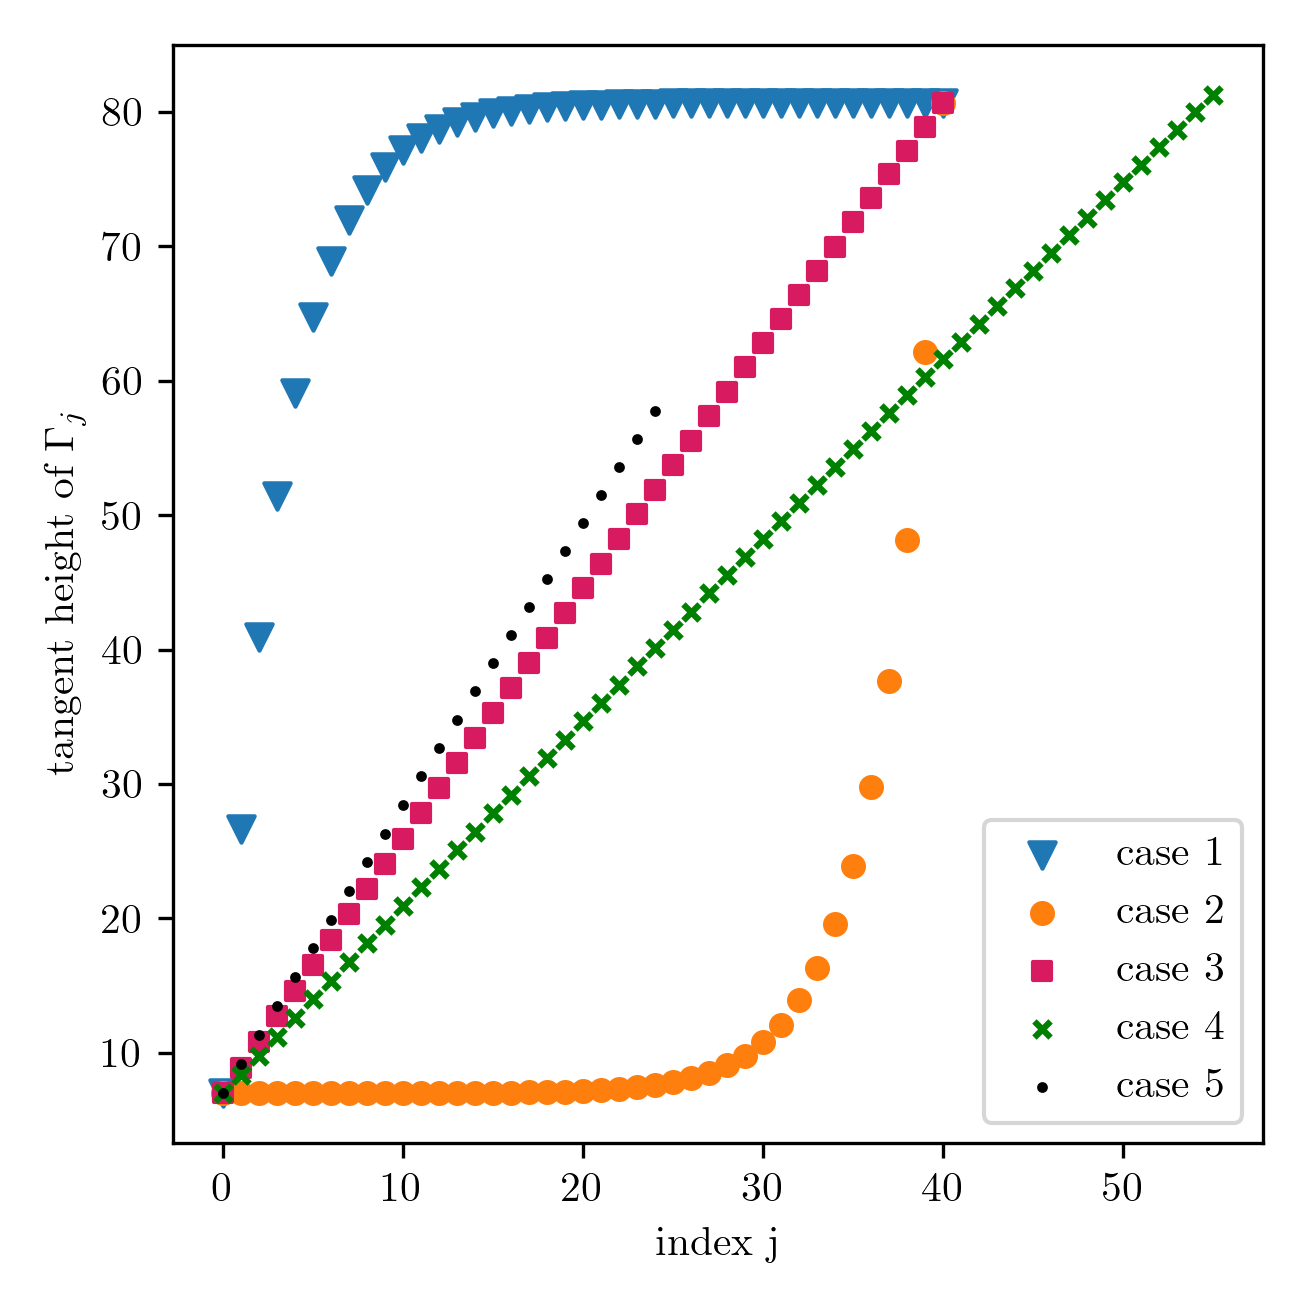
\includegraphics{MeasTangHeight.png}
	\caption[Tangent heights for different sequence of measurements.]{We plot the tangent heights for different cases of measurements.}
	\label{fig:TangHCases}
\end{figure}

Similar to a rpcial compontent ananlyis or ... we can find the singular value decompositon of $\bm{A}_L$ for ozone
\begin{align}
	\bm{A}_L = \bm{U} \bm{Sigma} \bm{V}
\end{align}
to anlayes where the forward model is sensitive and where not
we find the data space the image image space
linked by the isngular valiues nprojection

we dop that show that it donest matter how we emasure we wont get more information otu if the forward map.. it is deteminet by the measuremetn technique.

we can also adjust the number of measurement and find a suitable measurement set up


and show the limits of the meaduremts given a signal to noise ratio


\begin{figure}[ht!]
	\centering
	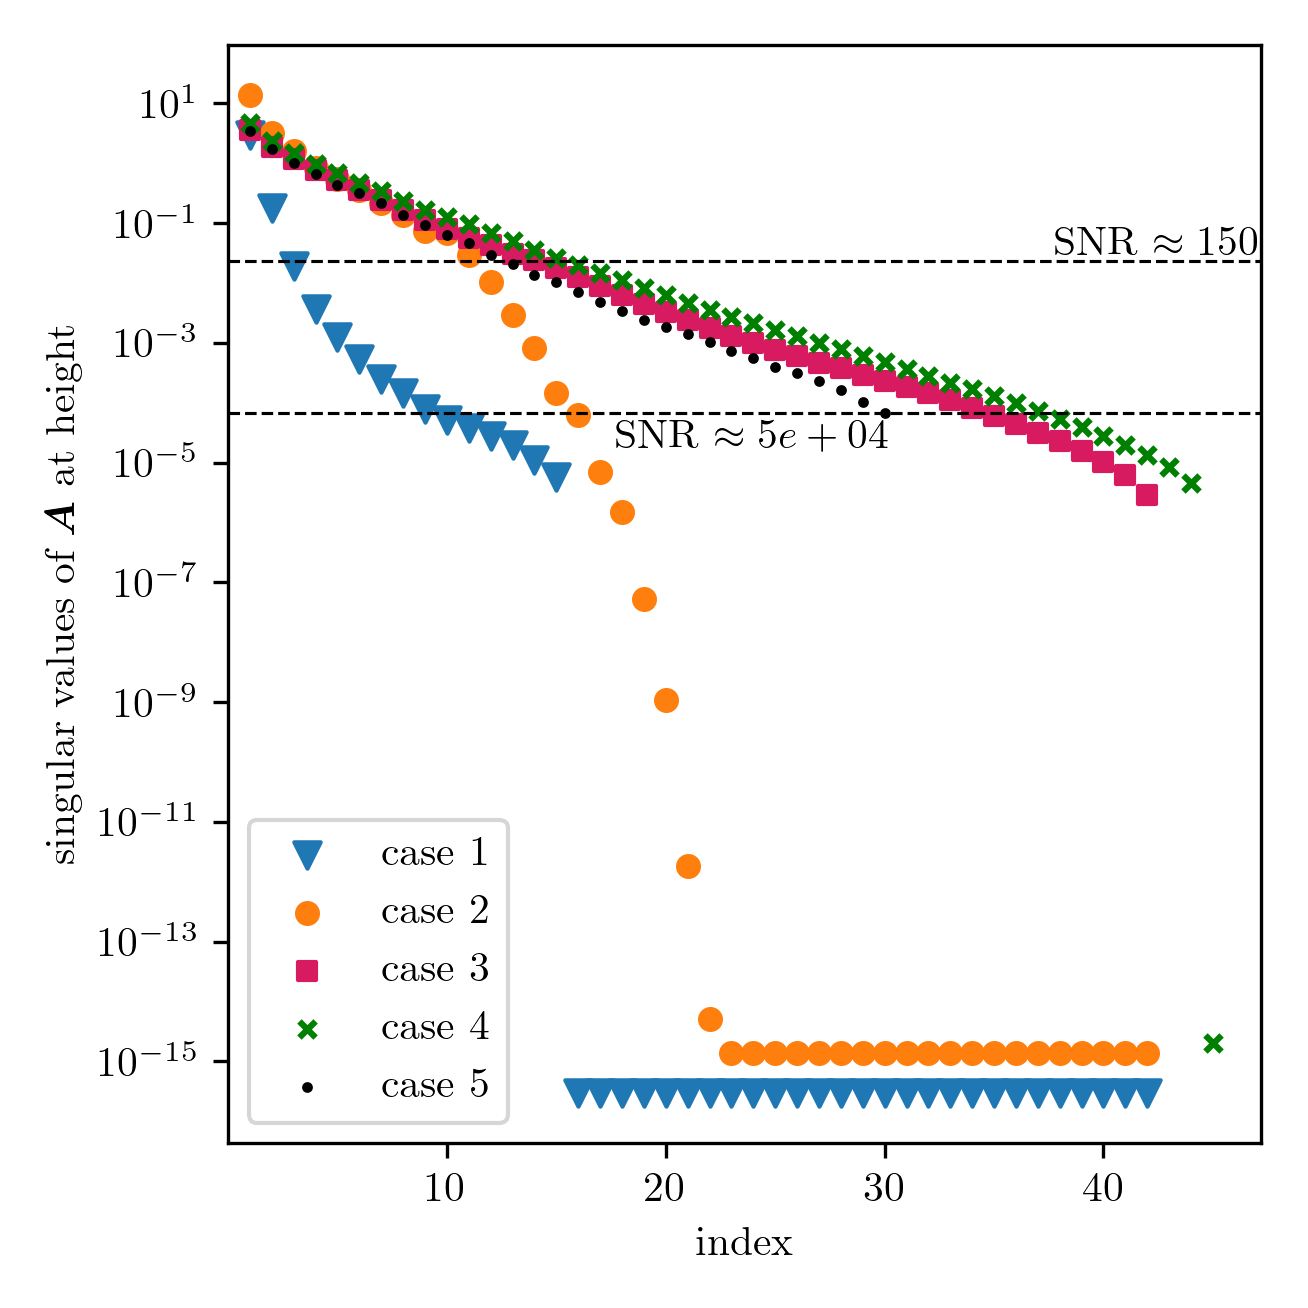
\includegraphics{SingValA.png}
	\caption[Singular values of linear forward model matrix for different sequences of measurements.]{We plot the singular values of linear forward model matrix for different sequences of measurements.
	The corresponding tangent heights of the different cases are plotted in Fig. \ref{fig:TangHCases}. We include an approximate for the disiered Signal to noise ratio if $s_1 \approx max(\bm{y}) $ the signal.}
	\label{fig:SingA}
\end{figure}


Not sensible in hght altidues
\begin{figure}[ht!]
	\centering
	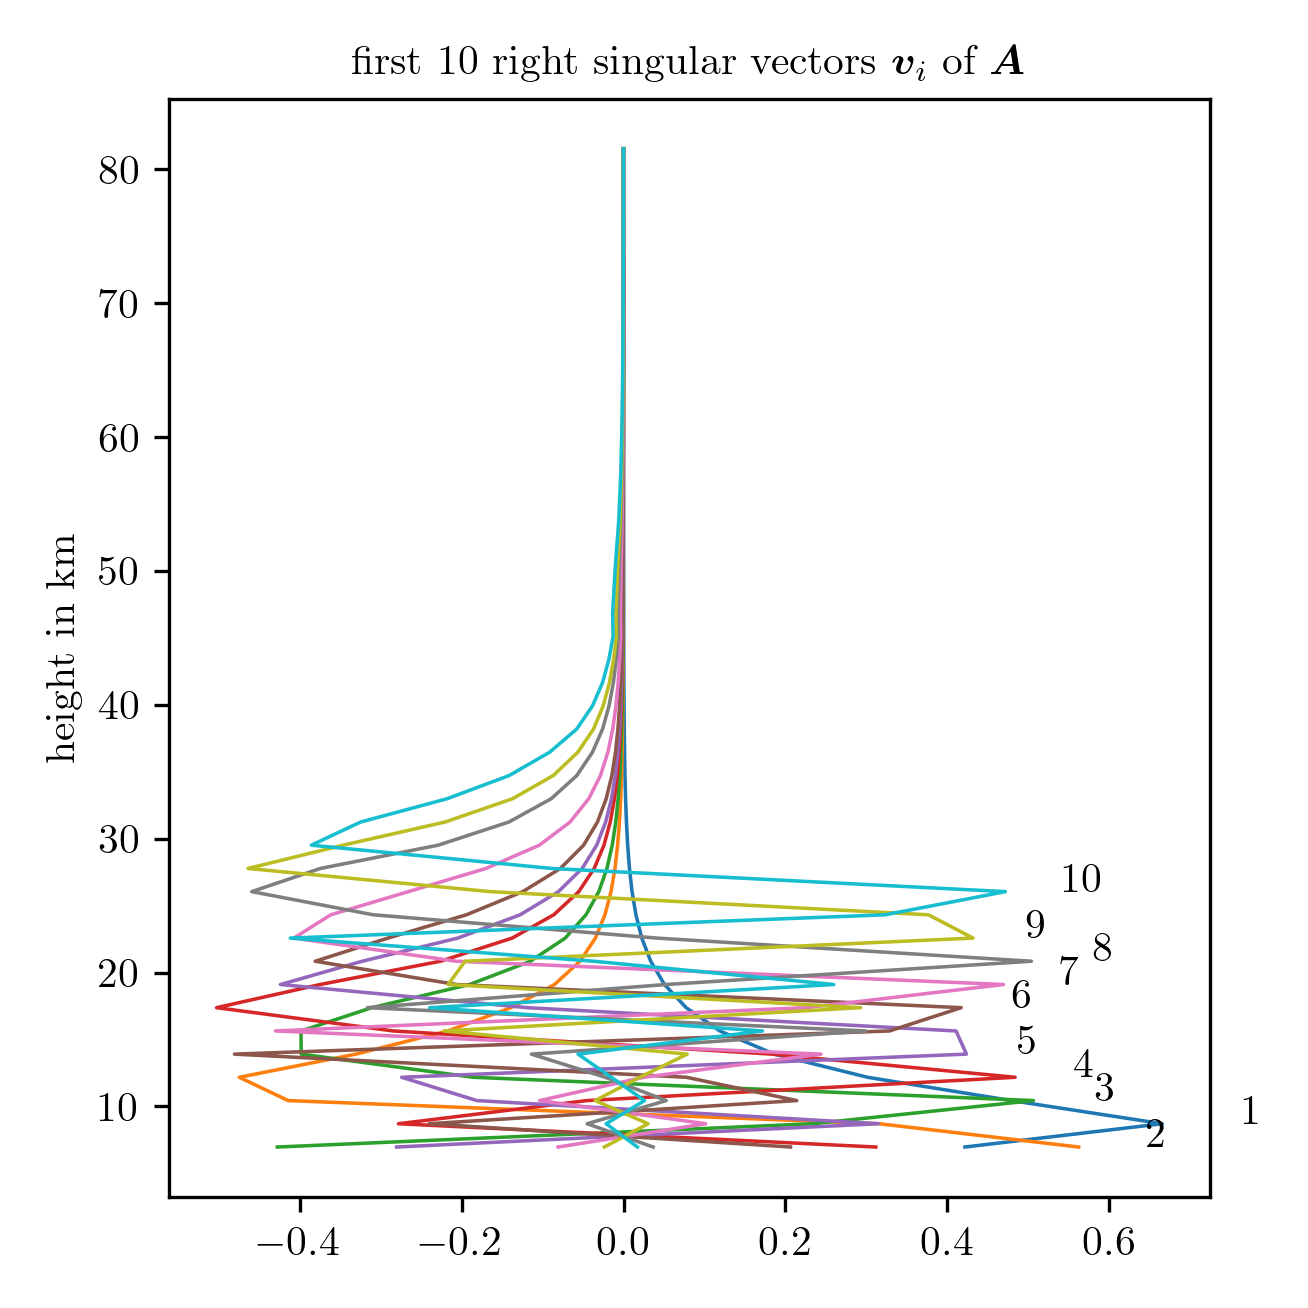
\includegraphics{SingVecA.png}
	\caption[Left singular vectors of forward model matrix for one sequence of measurements.]{We plot the first 20 left singular vectors of forward model matrix for case 5 sequence of measurements, see Fig. \ref{fig:SingA}.}
	\label{fig:SingVecA}
\end{figure}



%Hence, we can approximate the non-linear forward model $\bm{A}(\bm{x},  \bm{p},\bm{T})$ with a map $\bm{M}$ and the linear forward model $\bm{A}_L$, so that $\bm{A}(\bm{x},  \bm{p},\bm{T}) \approx \bm{M} \bm{A}_L $.
%Here, $\bm{A}_{L,j} $ of matrix $\bm{A}_L \in \mathbb{R}^{m \times n}$ is defined by the linear forward model, where absorption is neglected, e.g. set $\tau = 1$ in Eq.~\eqref{eq:absRTE}. 
%Then each entry in the row vector $\bm{A}_{L,j} $ is either defined by $ B(\nu) k(\nu)   \frac{\bm{p}}{k_{\text{B}} \bm{T}}  \text{d}r$ or $B(\nu) k(\nu)   \frac{\bm{x}}{k_{\text{B}}}  \text{d}r$, as in Eq.~\eqref{eq:RTE}.
%This poses a linear inverse problem with the forward map defined by the matrix $\bm{A} = \bm{M} \bm{A}_L$, where $\bm{M}$ is, more specifically, an affine map.


%\textcolor{red}{$h_{L,0}$ does not influences the values for $p_{L,O}/T_{L,0}$}
%\textcolor{red}{dont include bend of the line integral}

%\begin{figure}[ht!]
%	\centering
%	\scalebox{0.9}{\input{FirstLIMB.pdf_tex}}
%	\caption[General schematics of measurement setup]{This figure illustrates a limb-sounding measurement setup, specifically how the line of sight of a satellite at altitude $h_{\text{obs}}$ is partitioned according to a discretised atmospheric model. The atmosphere is divided into $n$ layers, allowing the line of sight $\Gamma_j$ to be discretised into segments $\Delta r_i$ for $i = \ell_j, \dots, n$.
%		Here, $\ell_j \in \mathbb{N}$ denotes the index corresponding to the tangent height $h_{\ell_j}$ relative to the Earth's radius $R_E$. This setup forms the basis for the numerical solution of the integral in Eq.~\ref{eq:RTE}, known as the radiative transfer equation.}
%	\label{fig:FirstLIMB}
%\end{figure}

%The absorption constant $k(\nu, T)$ for a single gas molecule at a specific wave number $\nu$ is calculated according to the HITRAN database \cite{gordon2022hitran2020} and acts as a source function when multiplied with the black body radiation $B(\nu,T)$, given by Planck`s law~\cite{rybicki2000rte}.
%We calculate the source function $B(\nu, T)$ and the absorption constant $ k(\nu, T)$ as follows.
%assumption local thermaodynamic equilibrium
%For one species at one specific wave-number the weighted absorption constant becomes
%\begin{align}
%	\overline{k(\nu, T, r)}    = \sum_{m=1}^{molec} k_m(\nu, T) x_m(r) =  k(\nu, T) x(r) \, ,
%\end{align}
%with the volume mixing ratio of ozone $x(r)$ at location $r$. 